\documentclass[11pt]{article}
\usepackage[colorlinks=true, allcolors=blue]{hyperref}
\usepackage{color}
\usepackage{amssymb}
\usepackage{amsmath}
\usepackage{tikz}
\usetikzlibrary{positioning}
\usepackage{xcolor}

\begin{document}

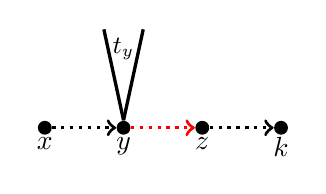
\begin{tikzpicture}
\tikzstyle{vertex}=[black,circle,fill,minimum size=5,inner sep=0pt]
\begin{scope}[every node/.style={vertex}]
 \node (x) at (-1,0) {};
 \node (y) at (0,0) {};
 \node (z) at (1,0) {};
 \node (k) at (2,0) {};
\end{scope}

\node[below] at (-1,0) {$x$};
\node[below] at (0,0) {$y$};
\node[below] at (1,0) {$z$};
\node[below] at (2,0) {$k$};
\draw[very thick,-] (y.north) to (0.25,1.25);
\draw[very thick,-] (y.north) to (-0.25,1.25);

\node at (0,1) {\small $t_y$};

\draw[very thick,dotted,->] (x.east) to (y.west);
\draw[very thick,dotted,->,red] (y.east) to (z.west);
\draw[very thick,dotted,->] (z.east) to (k.west);
\end{tikzpicture}

\end{document}